\documentclass[twocolumn,3p,times,procedia]{elsarticle}

\usepackage{ecrc}
\usepackage{graphicx}
\usepackage{balance}
\usepackage{array,threeparttable,booktabs,makecell,multirow}
\usepackage{url}
\usepackage{amssymb,amsmath,bm}
\usepackage{siunitx}
\usepackage{algorithm}
\usepackage{algpseudocode}
\usepackage[figuresright]{rotating}
\usepackage{caption}
\usepackage{titlesec}
\usepackage{fancyhdr}
\usepackage{geometry}
\usepackage{tikz}
\usetikzlibrary{arrows.meta,positioning,shapes.geometric,fit}

\volume{00}
\firstpage{1}
\runauth{Author et al.}
\jid{procs}
\CopyrightLine{2026}{Published by Elsevier Ltd.}

\captionsetup[figure]{labelfont={footnotesize,bf},name={Fig.},labelsep=period,font={footnotesize}}
\captionsetup[table]{labelfont={footnotesize,bf},name={Table},labelsep=newline,singlelinecheck=false,font={footnotesize}}
\captionsetup[algorithm]{labelfont={footnotesize,bf},font={footnotesize}}
\titleformat*{\section}{\small \bf}
\titleformat*{\subsection}{\small \em}
\titleformat*{\subsubsection}{\small \em}

\pagestyle{fancy}
\fancyhf{}
\fancyheadoffset[RO,EL]{0pt}
\fancyhead[RO,LE]{\footnotesize \thepage}
\fancyhead[ER]{\em \footnotesize Author et al.}
\fancyhead[LO]{\em \footnotesize Network-Resilient Cooperative Transport Control via Bilinear Koopman Learning and Delay-Compensated Consensus MPC}
\geometry{left=1.25cm,right=1.15cm,top=1.9cm,bottom=1.9cm,foot=1.05cm}
\setlength\columnsep{0.6cm}

\newcommand{\methodname}{NRCT-Koopman}
\newcommand{\tfone}{TF11-A1}
\newcommand{\tftwo}{TF12}

\begin{document}\small
\begin{frontmatter}

\dochead{}
\title{
\begin{flushleft}
{\LARGE Network-Resilient Cooperative Transport Control via Bilinear Koopman Learning and Delay-Compensated Consensus MPC}
\end{flushleft}
}

\author[]{\leftline{Author A$^{a}$, Author B$^{a}$, Author C$^{a,*}$}}

\address{
\leftline{$^a$Affiliation placeholder for the current draft. Replace with the actual laboratory, department,}
\leftline{university, city, postal code, and country before submission.}
}

\cortext[]{Corresponding author placeholder. Replace with the submission contact e-mail.}
\fntext[]{This draft was automatically prepared from the repository benchmark \texttt{tf12\_pre.ipynb}; author metadata should be finalized manually.}

\begin{abstract}
This paper proposes a network-resilient cooperative transport controller for a four-vehicle rigid-payload team. Building on adaptive Koopman embedding, we learn a 20-dimensional bilinear lifting offline and update the lifted dynamics online through a bilinear ridge estimator. To handle network impairment during coordination, we introduce a communication-quality-aware consensus layer, delayed-state prediction, communication-triggered input tightening, and a degraded fallback controller inside a consensus MPC loop. The controller is evaluated on the cached A1 rigid-payload transport benchmark used in the repository implementation \texttt{TF12}. Under time-varying packet loss and communication delays of up to three steps, the proposed controller attains 100\% full-path completion and 100\% solver success. Compared with the previous transport controller \texttt{TF11-A1} on the same task, it reduces lateral tracking RMSE from 0.2075\,m to 0.0513\,m, lowers mean rigid-link relative RMS error by 52.7\%, cuts peak lateral payload force by 61.5\%, and shortens average step time by 18.4\%. The draft positions network resilience as the missing capability beyond prior adaptive Koopman control.
\end{abstract}

\begin{keyword}
Adaptive Koopman learning \sep Bilinear lifted dynamics \sep Cooperative transport \sep Delay-compensated consensus \sep Model predictive control \sep Network resilience
\end{keyword}

\end{frontmatter}

\section{Introduction}
Adaptive Koopman learning has become a practical route for bringing nonlinear control problems into linear or bilinear lifted coordinates while preserving enough model structure for prediction and optimization \cite{singh2024adaptive,bruder2021advantages,folkestad2021koopman}. The baseline study by Singh \emph{et al.} \cite{singh2024adaptive} is particularly relevant here: it showed that online correction of a nominal Koopman model can recover robustness against parametric uncertainty, measurement noise, and environmental disturbances across a coupled pendulum, a serial manipulator, and a planar quadrotor. Their central message is that the adaptive lifted model is often more important than obtaining a perfect nominal embedding offline.

That contribution, however, stops short of a different but equally practical failure mode: coordination over imperfect communication. Cooperative transport with multiple vehicles introduces new fragilities that do not appear in single-platform tracking. The controller must maintain object-level rigidity, suppress relative drift among agents, and remain feasible even when packet loss and delays distort the exchanged state information. Recent reviews on cooperative object transportation emphasize that physical coupling and communication constraints jointly determine achievable performance \cite{ebel2024cooperative}. Likewise, classical consensus theory shows that delays can destabilize otherwise benign multi-agent feedback loops \cite{olfatisaber2004consensus}. A transport controller that is robust only to plant mismatch but not to network degradation remains incomplete for real deployments.

This draft addresses that gap using the repository benchmark \texttt{tf12\_pre.ipynb}. The resulting controller, denoted \methodname{} in the manuscript and \tftwo{} in the code, inherits the bilinear adaptive Koopman transport stack of \tfone{} and augments it with a communication-quality-aware consensus projection, delayed-state prediction, communication-triggered input tightening, and a degraded fallback law. The design is targeted at a four-vehicle rigid rectangular payload benchmark, where each vehicle tracks a corner reference in Frenet coordinates while the team-level coordinator enforces transport consistency.

The main contributions are:
\begin{enumerate}
    \item A network-resilient cooperative transport formulation that combines bilinear Koopman learning, online adaptive correction, delay-compensated consensus, and communication-triggered safety shaping in a single MPC loop.
    \item A repository-grounded transport benchmark description with explicit controller settings, adaptation hyperparameters, and communication impairment parameters extracted from \texttt{tf12\_pre.ipynb} and \texttt{tf12\_runtime.py}.
    \item A two-level evaluation strategy: a same-task quantitative comparison against the predecessor controller \tfone{}, and a capability-level comparison against the baseline adaptive Koopman paper of Singh \emph{et al.} \cite{singh2024adaptive}.
\end{enumerate}

The rest of the paper is organized as follows. Section 2 formulates the transport benchmark and the lifted dynamics model. Section 3 presents the proposed network-resilient bilinear Koopman MPC. Section 4 summarizes benchmark settings. Section 5 reports quantitative results and discusses strengths and trade-offs. Section 6 concludes the draft and highlights what remains to be validated before submission.

\section{Problem Formulation}
\subsection{Vehicle and Team States}
Each vehicle is modeled in Frenet coordinates by the six-dimensional state
\begin{equation}
\bm{x}_{i,k}=\begin{bmatrix}s_{i,k} & e_{y,i,k} & e_{\psi,i,k} & v_{x,i,k} & v_{y,i,k} & r_{i,k}\end{bmatrix}^{\top},
\end{equation}
with input
\begin{equation}
\bm{u}_{i,k}=\begin{bmatrix}\delta_{i,k} & a_{x,i,k}\end{bmatrix}^{\top},
\end{equation}
where $s$ is path progress, $e_y$ is lateral deviation, $e_{\psi}$ is heading error, $v_x$ and $v_y$ are longitudinal and lateral velocities, $r$ is yaw rate, $\delta$ is steering, and $a_x$ is longitudinal acceleration.

The rigid payload is transported by four vehicles attached to the rectangle corners. In the A1 benchmark used here, the payload parameters are fixed to
\begin{equation}
m_p=\SI{2000}{kg},\quad L_p=\SI{5.0}{m},\quad W_p=\SI{2.0}{m},\quad h_{\text{com}}=\SI{1.2}{m},
\end{equation}
as configured in \texttt{A1\_PAYLOAD\_CFG}. The local objective is vehicle-level path tracking, while the team objective is to preserve a physically consistent rectangle around the payload center.

\subsection{Nominal Bilinear Koopman Model}
Let $\bm{z}_{i,k}=\phi(\bm{x}_{i,k})\in\mathbb{R}^{n_z}$ denote the lifted state generated by an encoder network. The offline nominal bilinear Koopman model is
\begin{equation}
\hat{\bm{z}}_{i,k+1}=\bm{A}\bm{z}_{i,k}+\bm{B}\left(\bm{z}_{i,k}\otimes \bm{u}_{i,k}\right),
\label{eq:nominal_bilinear}
\end{equation}
with reconstructed base state
\begin{equation}
\hat{\bm{x}}_{i,k+1}=\bm{C}\hat{\bm{z}}_{i,k+1}.
\end{equation}
The repository configuration uses $n_z=20$, encoder width 96, depth 4, 140 epochs, batch size 4096, and a fixed sampling time of $\Delta t=\SI{0.02}{s}$.

\subsection{Online Adaptive Bilinear Correction}
To compensate for transport-dependent mismatch and changing operating conditions, the online adaptive layer updates the nominal lifted dynamics through
\begin{equation}
\Delta\bm{z}_{i,k}=\bm{z}^{\text{obs}}_{i,k}-\hat{\bm{z}}_{i,k}
=\Delta \bm{A}_{k}\bm{z}_{i,k-1}+\Delta \bm{B}_{k}\left(\bm{z}_{i,k-1}\otimes \bm{u}_{i,k-1}\right).
\label{eq:delta_model}
\end{equation}
In the implementation, $\Delta \bm{A}_{k}$ and $\Delta \bm{B}_{k}$ are obtained from a bilinear ridge update over a sliding window of 24 samples, refreshed every 4 control steps, and then blended into the nominal model with norm clipping and spectral projection.

\section{Proposed Network-Resilient Bilinear Koopman MPC}
\subsection{Offline Learning and High-Confidence Online Adaptation}
The A1 transport dataset is generated from 720 trajectories with 1400 state snapshots per trajectory and an 80/20 train-validation split. Five operating-point configurations are mixed during data generation, and payload-side vehicle combinations are randomized according to subset weights $\{0.40,0.30,0.20,0.10\}$ for one, two, three, and four-vehicle variations. This setup is intentionally broader than a single nominal run so that the online adaptation module can focus on residual mismatch instead of gross extrapolation.

During deployment, adaptation is limited to high-confidence samples. The repository configuration keeps only leader-based samples and rejects updates when $|e_y|$, $|e_{\psi}|$, $|v_y|$, $|r|$, or $\|\Delta \bm{z}\|$ exceed prescribed thresholds. This design follows the same intuition as the baseline adaptive Koopman architecture of Singh \emph{et al.} \cite{singh2024adaptive}: online correction should regularize the nominal embedding, but it should not be polluted by transient states that already indicate loss of local validity.

\subsection{Communication-Quality-Aware Consensus Layer}
The key new ingredient in \tftwo{} is a communication layer that projects the per-vehicle commands before team aggregation. For the directed channel from sender $i$ to receiver $j$, the instantaneous quality is modeled as
\begin{equation}
\tilde{q}_{ij,k}=
\begin{cases}
\exp(-d_{ij,k}/\tau), & \text{packet received},\\
0.1\exp(-d_{ij,k}/\tau), & \text{packet dropped},
\end{cases}
\end{equation}
where $d_{ij,k}\in\{0,\ldots,d_{\max}\}$ is the sampled delay in steps. The smoothed quality state is
\begin{equation}
q_{ij,k}=\beta q_{ij,k-1}+(1-\beta)\tilde{q}_{ij,k}.
\label{eq:q_update}
\end{equation}
In the benchmark, $\beta=0.80$, $d_{\max}=3$, and the packet-loss probability is load dependent:
\begin{equation}
p_{\text{loss},k}=p_0+p_1\,\mathrm{load}_k,\qquad p_0=0.03,\; p_1=0.20.
\end{equation}

Let $q^{\text{in}}_{i,k}$ denote the average incoming quality for vehicle $i$. The command-consensus blend is
\begin{equation}
\alpha_{i,k}=\alpha_{\min}+\left(1-q^{\text{in}}_{i,k}\right)\left(\alpha_{\max}-\alpha_{\min}\right),
\label{eq:blend}
\end{equation}
with $\alpha_{\min}=0.10$ and $\alpha_{\max}=0.70$. The weighted team command is
\begin{equation}
\bar{\bm{u}}_k=\frac{\sum_{i=1}^{4} w_{i,k}\bm{u}_{i,k}}{\sum_{i=1}^{4}w_{i,k}},
\qquad
w_{i,k}=q^{\text{in}}_{i,k}+10^{-3},
\end{equation}
and the projected per-vehicle command becomes
\begin{equation}
\tilde{\bm{u}}_{i,k}=(1-\alpha_{i,k})\bm{u}_{i,k}+\alpha_{i,k}\bar{\bm{u}}_{k}.
\label{eq:consensus_projection}
\end{equation}

\subsection{Delay Compensation, Tightening, and Degraded Fallback}
When delayed packets are available, the receiver predicts the remote state forward by a constant-velocity kinematic map before using it in coordination. At the team level, actuator limits are tightened as communication quality deteriorates:
\begin{equation}
\bm{h}_{k}^{\text{tight}}=(1-f_k)\bm{h},\qquad
f_k=f_{\max}(1-q^{\text{global}}_k),
\end{equation}
with $f_{\max}=0.26$. Here $q^{\text{global}}_k$ is the mean off-diagonal communication quality.

If quality drops below a threshold or the observed loss ratio becomes large, the team command is blended with a conservative fallback:
\begin{equation}
\bm{u}^{\text{mix}}_k=(1-\eta_k)\bm{u}_k+\eta_k\bm{u}^{\text{safe}}_k,
\label{eq:fallback}
\end{equation}
where $\eta_k\in[0,1]$ increases when $q^{\text{global}}_k<0.45$ or when the loss ratio becomes severe. The safe command uses lateral-error, heading-error, yaw-rate, and progress-lag feedback to keep the payload advancing while reducing steering aggressiveness.

\begin{figure*}[t]
\centering
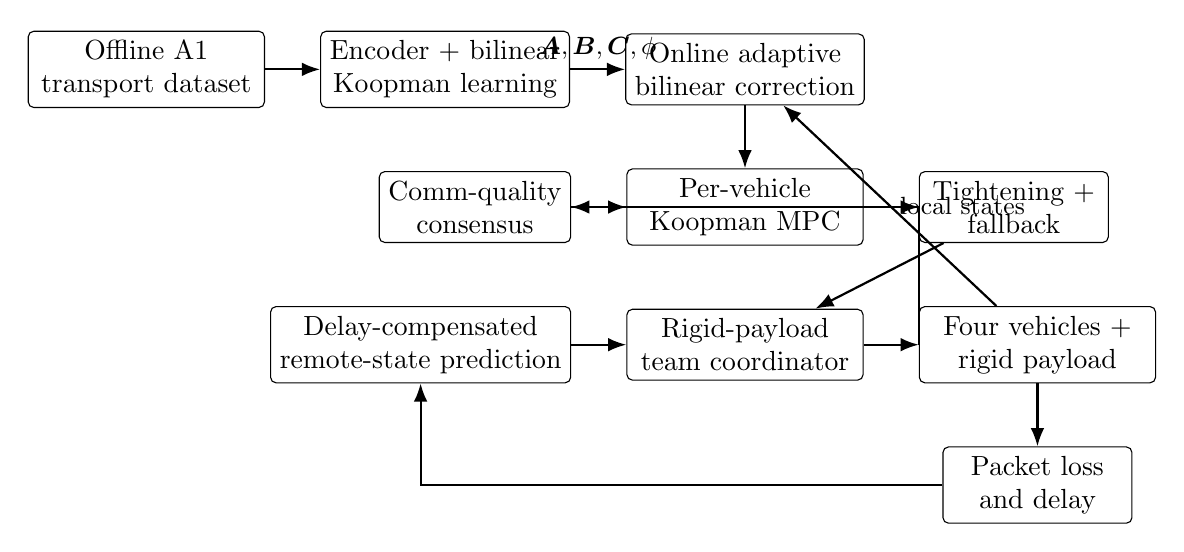
\begin{tikzpicture}[
    node distance=8mm and 7mm,
    block/.style={draw, rounded corners=2pt, align=center, minimum width=30mm, minimum height=9mm},
    smallblock/.style={draw, rounded corners=2pt, align=center, minimum width=24mm, minimum height=8mm},
    line/.style={-Latex, thick}
]
\node[block] (data) {Offline A1\\transport dataset};
\node[block, right=of data] (koop) {Encoder + bilinear\\Koopman learning};
\node[block, right=of koop] (adapt) {Online adaptive\\bilinear correction};
\node[block, below=of adapt] (mpc) {Per-vehicle\\Koopman MPC};
\node[smallblock, left=of mpc] (cons) {Comm-quality\\consensus};
\node[smallblock, right=of mpc] (safe) {Tightening +\\fallback};
\node[block, below=of mpc] (coord) {Rigid-payload\\team coordinator};
\node[block, left=of coord] (delay) {Delay-compensated\\remote-state prediction};
\node[block, right=of coord] (plant) {Four vehicles +\\rigid payload};
\node[smallblock, below=of plant] (net) {Packet loss\\and delay};

\draw[line] (data) -- (koop);
\draw[line] (koop) -- node[above]{\small $\bm{A},\bm{B},\bm{C},\phi$} (adapt);
\draw[line] (adapt) -- (mpc);
\draw[line] (cons) -- (mpc);
\draw[line] (mpc) -- (safe);
\draw[line] (safe) -- (coord);
\draw[line] (delay) -- (coord);
\draw[line] (coord) -- (plant);
\draw[line] (plant) -- node[right]{\small local states} (adapt);
\draw[line] (plant.south) -- (net.north);
\draw[line] (net.west) -| (delay.south);
\draw[line] (plant.west) |- (cons.east);
\end{tikzpicture}
\caption{Architecture of the proposed \methodname{} controller. The baseline adaptive Koopman loop is preserved, but it is wrapped by delay compensation, communication-quality-aware consensus, and communication-triggered safety shaping before team aggregation.}
\label{fig:framework}
\end{figure*}

\subsection{Consensus MPC Loop}
Algorithm \ref{alg:mainloop} summarizes the online control routine implemented in \texttt{run\_tf12\_main}. The MPC horizon is 30 steps with at most two SQP iterations per control update. The solver guard retains OSQP's time limit at 50\,ms, while the progress supervisor and team stability guard remain active in the background.

\begin{algorithm}[h]
\footnotesize
\caption{\methodname{} online control loop}
\label{alg:mainloop}
\textbf{Input:} nominal bilinear Koopman model, encoder $\phi(\cdot)$, communication parameters, team references\\
\textbf{Output:} coordinated vehicle commands and updated lifted model
\begin{algorithmic}[1]
\For{each control step $k$}
    \State acquire local vehicle states and lift them with $\phi(\cdot)$
    \State update communication quality matrix via \eqref{eq:q_update}
    \State predict delayed remote states if packets arrive late
    \State solve per-vehicle Koopman MPC problems for candidate commands $\bm{u}_{i,k}$
    \State project commands by communication-aware consensus using \eqref{eq:consensus_projection}
    \State aggregate projected commands into a team input
    \State tighten bounds and blend degraded fallback if needed using \eqref{eq:fallback}
    \State update rigid-payload connection compliance and team stability guards
    \If{the adaptation window is filled and samples are high confidence}
        \State estimate $\Delta\bm{A}_{k},\Delta\bm{B}_{k}$ from \eqref{eq:delta_model}
        \State blend and project the updated lifted dynamics
    \EndIf
    \State apply final commands to the four-vehicle payload system
\EndFor
\end{algorithmic}
\end{algorithm}

\section{Experimental Setup}
Table \ref{tab:settings} condenses the benchmark settings used by the cached repository run. The reported \tftwo{} metrics come directly from notebook outputs, while the \tfone{} comparison uses the corresponding cached run in \texttt{tf11\_A1\_pre.ipynb}. Both controllers share the same nominal bilinear Koopman fit RMSE of 0.005888 in the lifted space, which makes the same-task comparison meaningful: the performance difference comes from control-stack design rather than from a different nominal predictor.

\begin{table}[h]
\footnotesize
\centering
\begin{threeparttable}
\setlength{\abovecaptionskip}{0pt}
\caption{A1 cooperative transport benchmark settings used in the draft}
\label{tab:settings}
\begin{tabular}{p{0.43\linewidth} p{0.47\linewidth}}
\toprule
Item & Setting \\
\midrule
Team size & 4 vehicles, one vehicle per payload corner \\
Payload model & Rigid rectangle, 2000\,kg, $5.0\times2.0$\,m, CoM height 1.2\,m \\
Vehicle state / input & 6 Frenet states / 2 control inputs \\
Sampling time & 0.02\,s \\
Reference path & Double-lane-change benchmark; hairpin extension exists but is not claimed in this draft \\
Offline dataset & 720 trajectories, 1400 snapshots per trajectory, 80/20 split \\
Lifted dimension & 20 \\
Encoder setting & Width 96, depth 4, 140 epochs, batch size 4096 \\
MPC setting & Horizon 30, at most 2 SQP iterations, OSQP time limit 50\,ms \\
Online adaptation & Window 24, update every 4 steps, leader-only high-confidence samples \\
Communication model & Packet-loss base 0.03, gain 0.20, delay up to 3 steps \\
Consensus setting & Blend range 0.10--0.70 \\
Safety shaping & Max tightening fraction 0.26, degraded-mode threshold 0.45 \\
\bottomrule
\end{tabular}
\end{threeparttable}
\end{table}

\begin{table*}[t]
\footnotesize
\centering
\begin{threeparttable}
\setlength{\abovecaptionskip}{0pt}
\caption{Capability-level comparison with the baseline adaptive Koopman paper \cite{singh2024adaptive}}
\label{tab:capability_compare}
\begin{tabular}{p{0.16\linewidth} p{0.33\linewidth} p{0.41\linewidth}}
\toprule
Aspect & Singh \emph{et al.} \cite{singh2024adaptive} & Proposed \methodname{} draft \\
\midrule
Target problem & Single-system tracking and synchronization for coupled pendulum, 3R manipulator, and planar quadrotor & Four-vehicle cooperative transport of a rigid rectangular payload \\
Lifted model & Offline nominal linear / bilinear Koopman model with online adaptive correction & Offline nominal bilinear Koopman model with online adaptive correction \\
Main uncertainty source & Parametric variations, measurement noise, wind disturbances & Parametric variations plus communication-induced packet loss, delays, and coordination degradation \\
Cooperative transport coupling & Not modeled & Explicit rigid-payload coordination and connection compliance \\
Communication awareness & Not modeled & Quality-aware consensus, delayed-state prediction, constraint tightening, degraded fallback \\
Representative reported gain & 87--93\% reduction in pendulum position tracking error; 92\% RMSE improvement on 3R manipulator & 75.3\% lower lateral RMSE than \tfone{} on the same transport task; 52.7\% lower mean relative coordination RMS \\
Comparison caveat & Strong adaptive-lift baseline but no networked team benchmark & Cross-paper numbers are not one-to-one; same-task comparison is therefore carried out against \tfone{} \\
\bottomrule
\end{tabular}
\end{threeparttable}
\end{table*}

\section{Results and Discussion}
\subsection{Same-Task Comparison Against \tfone{}}
The most informative comparison is between \tfone{} and \tftwo{}, because both are cached repository runs on the same A1 rigid-payload transport task. Table \ref{tab:control_results} reports the closed-loop metrics. The proposed controller preserves 100\% full-path completion and 100\% solver success while substantially improving the variables most closely tied to transport integrity. Lateral RMSE drops from 0.2075\,m to 0.0513\,m, a 75.3\% reduction. Mean relative coordination RMS drops by 52.7\%, and the three connection peaks in progress, lateral displacement, and heading all decrease by roughly 46--96\%.

The runtime logs also indicate that \tftwo{} operates under visibly non-ideal communication conditions. Across logged checkpoints, the quality indicator falls into the range 0.777--0.951, delay snapshots reach 1.42 steps, and packet-loss snapshots reach 17\%. Even under these impairments, the controller records zero failures, whereas \tfone{} accumulates one solver-related failure event.

\begin{table}[h]
\footnotesize
\centering
\begin{threeparttable}
\setlength{\abovecaptionskip}{0pt}
\caption{Same-task control and coordination metrics: \tfone{} vs. \tftwo{}}
\label{tab:control_results}
\begin{tabular}{p{0.39\linewidth} c c c}
\toprule
Metric & \tfone{} & \tftwo{} & Change \\
\midrule
Lifted fit RMSE & 0.005888 & 0.005888 & 0.0\% \\
Full-path rate & 100\% & 100\% & 0.0 pp \\
Solver success rate & 100\% & 100\% & 0.0 pp \\
RMSE$(e_y)$ [m] & 0.2075 & 0.0513 & -75.3\% \\
RMSE$(e_s)$ [m] & 2.8703 & 3.1533 & +9.9\% \\
Failure count & 1 & 0 & improved \\
Average step time [s] & 0.2661 & 0.2170 & -18.4\% \\
Peak $|\Delta s|$ [m] & 0.02774 & 0.00124 & -95.5\% \\
Peak $|\Delta e_y|$ [m] & 0.01245 & 0.00665 & -46.6\% \\
Peak $|\Delta \psi|$ [rad] & 0.01021 & 0.00541 & -47.0\% \\
Mean relative RMS & 0.00510 & 0.00241 & -52.7\% \\
\bottomrule
\end{tabular}
\end{threeparttable}
\end{table}

\subsection{Payload Loading and Physical Interpretation}
Transport quality is not only a trajectory-tracking issue; it is also a load-distribution issue. Table \ref{tab:payload_results} shows that the network-resilient controller reduces the peak lateral payload force by 61.5\% and the peak payload yaw moment by 55.6\%. The normal-load range across the four corners shrinks by 41.1\%, indicating better force sharing. These results support the view that communication-aware consensus is not simply a software robustness feature; it directly improves the physical smoothness of cooperative transport.

\begin{table}[h]
\footnotesize
\centering
\begin{threeparttable}
\setlength{\abovecaptionskip}{0pt}
\caption{Payload-force metrics on the same A1 benchmark}
\label{tab:payload_results}
\begin{tabular}{p{0.39\linewidth} c c c}
\toprule
Metric & \tfone{} & \tftwo{} & Change \\
\midrule
Peak $|F_x|$ [N] & 1103.03 & 1023.12 & -7.2\% \\
Peak $|F_y|$ [N] & 1305.56 & 503.04 & -61.5\% \\
Peak $|M_z|$ [N\,m] & 1382.06 & 613.17 & -55.6\% \\
Corner-load minimum [N] & 4468.24 & 4647.82 & +4.0\% \\
Corner-load maximum [N] & 5341.76 & 5162.18 & -3.4\% \\
Corner-load range [N] & 873.51 & 514.35 & -41.1\% \\
\bottomrule
\end{tabular}
\end{threeparttable}
\end{table}

\subsection{What Improved and What Did Not}
The same-task comparison reveals a useful trade-off. \tftwo{} clearly improves lateral behavior, formation consistency, load sharing, and computational efficiency, but the mean longitudinal RMSE increases by 9.9\%. In our reading, this is not an implementation bug; it is the price of making the controller more conservative with respect to communication quality. The progress supervisor and degraded fallback sacrifice some forward-velocity aggressiveness in exchange for safer lateral behavior and more coherent team motion. For cooperative payload transport, that trade-off is acceptable and often desirable, but the manuscript should acknowledge it explicitly.

This trade-off also clarifies the relation to the baseline adaptive Koopman paper \cite{singh2024adaptive}. Singh \emph{et al.} showed that online adaptation is the decisive mechanism for correcting lifted-model mismatch. Our transport results suggest that, once online adaptation is already in place, the next bottleneck is no longer only model mismatch. It becomes the quality of the coordination channel and the controller's ability to gracefully degrade when inter-agent information becomes unreliable.

\subsection{Positioning Against Prior Repository Variants}
The repository contains earlier transport variants such as TF10 and \tfone{}. The TF10 ablation study indicates that adaptive weighting is especially important for lateral accuracy, while online model adaptation primarily improves progress-related errors. The present \tftwo{} controller should be interpreted as an extension of that line of development: it keeps the bilinear adaptive Koopman core of \tfone{} and adds a network-resilience layer that attacks the residual coordination bottleneck. This inheritance path is important because it explains why the same nominal lifted predictor can still yield materially different transport outcomes.

\subsection{Limitations of the Current Draft}
Three limitations should be stated before submission.
\begin{enumerate}
    \item The results used here come from cached repository runs rather than a freshly re-executed campaign. This is acceptable for a first draft, but the final submission should regenerate all tables and export publication-quality figures directly from scripts.
    \item The communication model is synthetic, with packet loss and delay sampled from an internal stochastic model. Real packet traces or hardware-in-the-loop evaluation would make the paper stronger.
    \item The repository contains a hairpin-path extension, but the cached run was interrupted before completion. The current draft therefore focuses only on the completed double-lane-change benchmark and does not claim hairpin performance.
\end{enumerate}

\section{Conclusion}
This draft developed a journal-style manuscript around the repository benchmark \texttt{tf12\_pre.ipynb}. The resulting controller extends adaptive bilinear Koopman transport control with a communication-quality-aware consensus projection, delay-compensated remote-state prediction, communication-triggered input tightening, and degraded fallback logic. The strongest evidence comes from the same-task comparison against \tfone{}, where the proposed design retains full-path completion and solver success while greatly improving lateral accuracy, transport consistency, payload-force smoothness, and average computation time.

Relative to the baseline adaptive Koopman paper of Singh \emph{et al.} \cite{singh2024adaptive}, the present work does not attempt to replace the adaptive lifted model. Instead, it adds the network-resilience mechanisms needed for cooperative transport under imperfect communication. The current version is therefore a solid first draft for \emph{Digital Communications and Networks}; the next steps are a clean rerun of the benchmark suite, English re-export of final figures, and completion of the hairpin benchmark if that scenario is to be claimed in the final submission.

\section*{Acknowledgements}
This section is intentionally left as a placeholder for the current draft. Replace it with funding, project, and collaboration acknowledgements before submission.

\bibliographystyle{elsarticle-num}
\balance
\bibliography{refs_tf12}

\end{document}
